% Commented out: 
% \addbibresource
% \includepdf

\documentclass[12pt,letterpaper,english,bibliography=totocnumbered, abstract=on]{scrartcl}

\usepackage{indentfirst}
\usepackage[titletoc]{appendix}
\usepackage{fullpage}
%\usepackage{subfiles}
\usepackage[T1]{fontenc}
\usepackage[latin9]{inputenc}
\usepackage{color}
\usepackage{babel}
\usepackage{verbatim}
\usepackage[unicode=true,pdfusetitle,
bookmarks=true,bookmarksnumbered=false,bookmarksopen=false,
breaklinks=true,pdfborder={0 0 0},pdfborderstyle={},backref=false,colorlinks=true]
{hyperref}
\hypersetup{linkcolor=blue,citecolor=blue,urlcolor=blue}

\usepackage{booktabs}
\usepackage{multirow}
\usepackage{adjustbox}
\usepackage{threeparttable}
\usepackage[table]{xcolor}
\usepackage{csquotes}
\usepackage{soul} % for hiliting text: \hl

\usepackage[backend=biber, style=authoryear, maxbibnames=99, dashed=false]{biblatex}
\setlength\bibitemsep{2\itemsep}
%\addbibresource{mylibrary.bib}
%\addbibresource{CRB.bib}

\usepackage{pdfpages}
\usepackage{float} % Allows use of H to place floats

\usepackage{pgfgantt}

\usepackage{framed}

% Prevent page breaks within paragraphs
% https://tex.stackexchange.com/questions/21983/how-to-avoid-page-breaks-inside-paragraphs
\widowpenalties 1 10000

\begin{document}

\titlehead{Technical Report}

\title{\textit{Aulacaspis yasumatsui} on \textit{Cycas micronesica} Growing Outside the Conservation Plots on Tinian}

\author{Aubrey Moore}

\date{March 23, 2022\\Revised March 23, 2022}

\maketitle
%\footnote{\url{https://github.com/aubreymoore/2020-FS-CRB-biocontrol-project/blob/master/combined-proposal.pdf}}
\newpage
\tableofcontents

\pagebreak

\section{Introduction}

The most recent version of this document may be downloaded from \url{https://github.com/aubreymoore/Tinian-cycad-images/raw/main/report/tinian_cycad_images.pdf}.

\begin{figure}[h]
	\centering
	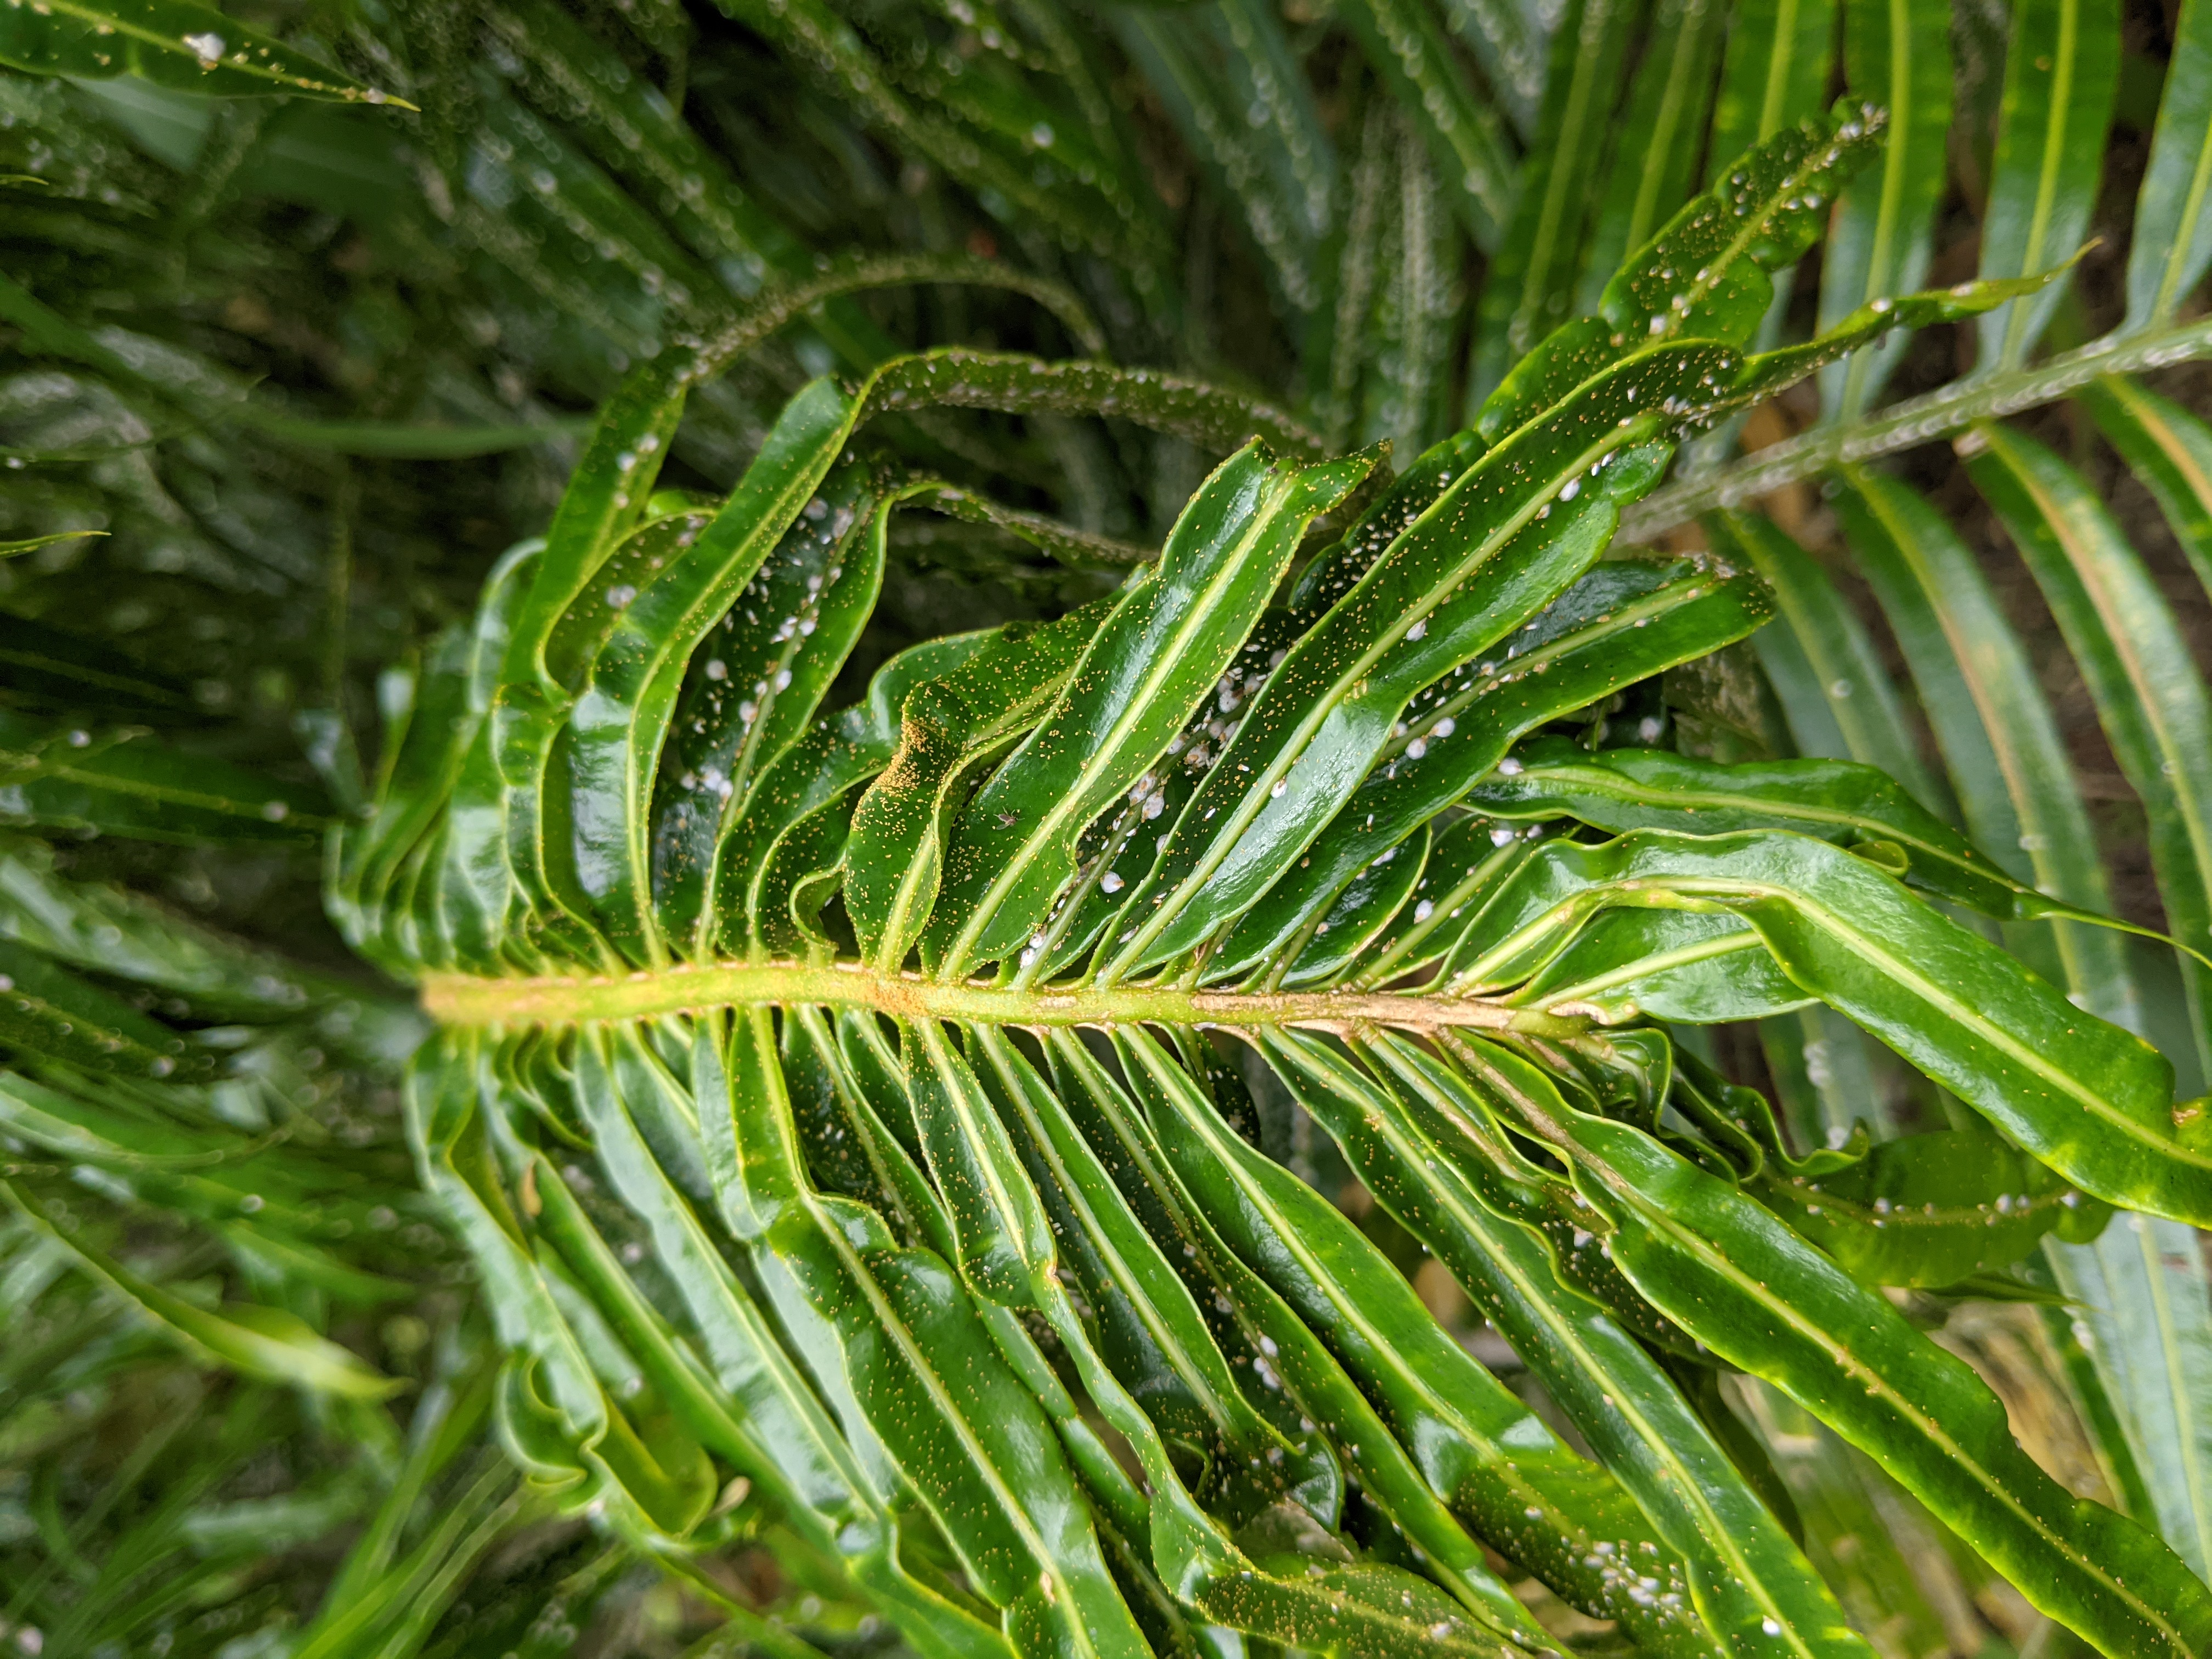
\includegraphics[width=1\linewidth]{../images/PXL_20210725_040405506}
	\caption{This image of \textit{Cycas micronsesica} leaflets infested with CAS was taken by Ken Puliafico on Mount Lasu, Tinian on March ?? 2022. It is remarkable because large numbers of scale crawlers are clearly visible.}
	\label{fig:crawlers}
\end{figure}


\section{Web map}

\url{https://aubreymoore.github.io/Tinian-cycad-images/webmap/webmap/}

%\section{Combined Budget}
%
%% Please add the following required packages to your document preamble:
%% \usepackage{booktabs}
%% \usepackage[table,xcdraw]{xcolor}
%% If you use beamer only pass "xcolor=table" option, i.e. \documentclass[xcolor=table]{beamer}
%\begin{table}[h]
%	\centering
%	\begin{tabular}{@{}lrrr@{}}
%		\toprule
%		\multicolumn{1}{c}{\textbf{Item}} & \multicolumn{1}{c}{\textbf{Cost(UOG)}} & \multicolumn{1}{c}{\textbf{Cost(GDOA)}} & \multicolumn{1}{c}{\textbf{Total}} \\ 
%		\midrule
%		Personnel & \$83,463 & \$72,987 & \$156,450 \\
%		Benefits  & \$19,196 & \$5,584 & \$24,780 \\
%		Travel & \$4,000 & \$0 & \$4,000 \\
%		Supplies & \$0 & \$2,545 & \$2,545 \\ 
%		\midrule
%		\multicolumn{1}{r}{\textbf{SUBTOTAL}} & \textbf{\$106,659} & \textbf{\$81,116} & \textbf{\$187,775} \\ \midrule
%		Administrative fee & \$15,999 & \$12,167 & \$28,166 \\ \midrule
%		\multicolumn{1}{r}{\textbf{TOTAL}} & \textbf{\$122,658} & \textbf{\$93,283} & \textbf{\$215,941} \\ \bottomrule
%	\end{tabular}
%\end{table}
%
%\begin{description}
%	
%	\item [{Personnel (UOG)}] includes salary for an insect pathologist (Dr. James Grasela, 1 FTE, \textbf{\$64,000}) and salary for a technician \textbf{\$19,463}.
%	\textbf{Total=\$83,463}.
%	
%	\item [{Benefits (UOG)}] benefits calculated at 23\%*\$83,463=\textbf{\$19,196}.
%
%	\item [{Personnel (GDOA)}] Research Associate I, (fulltime, \$20.34/hour, 2080hrs)=\textbf{\$42,307}; 
%	Research Assistant III (fulltime or 2x halftime, \$14.75/hour, 2080hrs)=\textbf{\$30,680}. Total=\textbf{\$72,987}.
%	
%	\item [{Benefits (GDOA)}] Social Security and Medicare (7.65\%*\$72,987)=\textbf{\$5,584}.
%	
%	\item [{Travel (UOG)}] includes airfare and other relocation expenses for Dr. Grasela who resides in Missouri.
%	
%	\item [{Supplies (GDOA)}]  
%	Fuel (7,488miles, work truck, 20MPG, \$4.50/gallon)=\textbf{\$1,685}; 
%	Survey Supplies (peanut butter, chopsticks, fluorescent tape/flags, ziplock bags)=\textbf{\$500}; 
%	Wrist Garmin GPS units (2x \$180)=\textbf{\$360}. \textbf{Total=\$2,545}.	
%	
%	\item [{Administrative~fee (UOG and GDOA)}] 15\% of direct costs
%	is charged by the Research Corporation of the University of Guam for
%	services provided. 
%	
%\end{description}
%
%
%\pagebreak
%\section{Little Fire Ant Management}
%Please see next page.
%
%%\includepdf[pages=-]{LFA-proposal.pdf}
%
%\section{Coconut Rhinoceros Beetle Biological Control}
%Please see next page.
%
%If you want to use active hyperlinks in the attached document, please download from 
%\tiny{\url{https://github.com/aubreymoore/2020-FS-CRB-biocontrol-project/blob/master/combined-proposal.pdf}}
%
%%\includepdf[pages=-]{proposal.pdf}
%
%\newpage{}
%\begin{appendices}
%	
%\section{Form SF-424 (Revised May 5, 2021)}
%Please see next page.
%%\includepdf[pages=-]{forms/25k-increase/SF-424-signed.pdf}
%
%\section{Form SF-424A (Revised May 4, 2021)}
%Please see next page.
%%\includepdf[pages=-]{forms/25k-increase/SF-424A-filled.pdf}
%
%\section{Form AD-1047}
%Please see next page.
%%\includepdf[pages=-]{forms/AD1047-signed.pdf}
%
%\section{Form AD-1049}
%Please see next page.
%%\includepdf[pages=-]{forms/AD1049-signed.pdf}
%
%\section{Form SF-LLL}
%Please see next page.
%%\includepdf[pages=-]{forms/LLL-signed.pdf}
%
%\section{Form FS-1500-22A}
%Please see next page.
%%\includepdf[pages=-]{forms/FS1500-22A-signed.pdf}
%
%\end{appendices}

\end{document}
